\documentclass{beamer}

\usepackage{amssymb}
\usepackage{fancyvrb}
\usepackage{stmaryrd}
\usepackage{graphicx}
\usefonttheme{serif}


\newcommand{\Nat}{\mathbb{N}}

\SaveVerb{zer}=Z=
\SaveVerb{suc}=Succ n=
\SaveVerb{thr}=Succ (Succ (Succ Z))=
\SaveVerb{ele}=Succ (Succ (Succ (Succ (Succ (Succ (Succ (Succ (Succ (Succ (Succ Z))))))))))=
\SaveVerb{enn}=n=

\title{What About the Natural Numbers?}%\texorpdfstring{$\mathbb{N}$}}
\subtitle{JMCT}
\date{}

\usetheme{jmct}

\usepackage{calc}

\newcommand{\textover}[3][l]{%
 % #1 is the alignment, default l
 % #2 is the text to be printed
 % #3 is the text for setting the width
 \makebox[\widthof{#3}][#1]{#2}%
 }

\newcommand{\blueit}[1]{%
  {\color{dark-lucid-blue}#1}%
}
\newcommand{\blueite}[1]{%
  \blueit{\emph{#1}}%
}


\newcommand{\myquote}[3]{
  ``#1''
  \vspace{3pt}
  \hrule
  \begin{flushright}
  --- \blueit{\emph{#2}}, \emph{#3}
  \end{flushright}
}

\begin{document}
	\frame {
		\titlepage
	}

%%%%%%%%%%%%%%%%%%%%%%%%%%%%%%%%%%%%%%%% 
%%% Intro
%%%%%%%%%%%%%%%%%%%%%%%%%%%%%%%%%%%%%%%% 

  \frame {
    \centering {\fontsize{88}{68}\selectfont $\mathbb{N}$\phantom{?}}
  }
  \frame {
    \centering {\fontsize{88}{68}\selectfont $\mathbb{N}$?}
  }


  \frame {
    \myquote{Some thirty years into the history of
      machine-independent programming language design, the treatment of numbers
      is still problematic.}{Colin Runciman}{1989}
  }
  \frame {
    \myquote{Some \textover[c]{\blueit{sixty}}{thirty} years into the history of
      machine-independent programming language design, the treatment of numbers
      is still problematic.}{Me}{just now}
  }
  \frame{
    \frametitle{Main takeaway}
    The number system we use should relate to the structures of the problem
    we're solving.
  }
  \frame{
    \frametitle{Main takeaway}
    For some domains, the use of Reals\footnote{or their approximation via
    \texttt{Float}s} may be appropriate:
    \begin{itemize}
      \item<2 -> e.g. physics calculations involving volume, speed, or mass
    \end{itemize}
  }
  \frame{
    \frametitle{Main takeaway}
    For \emph{many} problems \blueit{Integers} are appropriate:
    \begin{itemize}
      \item<2 -> Fixed-precision DSP
      \item<3 -> Bank account balance :'(
    \end{itemize}
  }
  \frame{
    \frametitle{Main takeaway}
    Runciman's argument:\newline
    \hangindent=0.7cm
    For many of the discrete structures involved in the
    day-to-day practice of programming, the \blueit{natural} numbers are
    the most appropriate number system.
  }
  \frame{
    \frametitle{How?}
    In the process of exploring the Natural Numbers, we'll be developing an API.
    As we progress we'll see how different representations affect our API.
  }

%%%%%%%%%%%%%%%%%%%%%%%%%%%%%%%%%%%%%%%% 
%%% Outline
%%%%%%%%%%%%%%%%%%%%%%%%%%%%%%%%%%%%%%%% 

      %* Overview of the $\mathbb{N}$s themselves
      %* Programming with \texttt{Nat}
      %* Arithmetic with \texttt{Nat} and properties we care about
      %* How does \texttt{Nat} influence API design?
      %* Implementation Concerns
      %* Beyond \texttt{Nat}
      %* Conclude

  %%%%%%%
  % Goals
  %
  \frame{
    \frametitle{\#goals}
    \begin{enumerate}
      \item<2 -> Show you that the [lazy?] $\mathbb{N}$s are \blueite{Good}
                 and \blueite{Proper}
      \item<3 -> Demonstrate that even \emph{simple} choices of types
                 for an API have deep consequences
      \item<4 -> Have you asking ``What about the Natural Numbers?''
                 next time you create an API.
    \end{enumerate}
  }
  %%%%%%%
  % Actual Outline
  %
  \frame{
    \frametitle{Shape of things to come}
    \begin{enumerate}
      \item<2 -> Overview of the $\mathbb{N}$s themselves
      \item<3 -> Programming with \texttt{Nat}
      \item<4 -> Arithmetic with \texttt{Nat} and properties we care about
      \item<5 -> How does \texttt{Nat} influence API design?
      \item<6 -> Implementation concerns
      \item<7 -> Beyond \texttt{Nat}
      \item<8 -> Conclude
    \end{enumerate}
  }

  %%%%%%%
  % What are they?
  %
  % We actually see them here! We just counted things, _that's_
  % the natural number.
  \frame{
    \frametitle{Let's start}
    \begin{enumerate}
      \item \blueit{Overview of the $\mathbb{N}$s themselves}
      \item Programming with \texttt{Nat}
      \item Arithmetic with \texttt{Nat} and properties we care about
      \item How does \texttt{Nat} influence API design?
      \item Implementation concerns
      \item Beyond \texttt{Nat}
      \item Conclude
    \end{enumerate}
  }

  \frame{
    \frametitle{What \emph{are} they?}
    The \emph{Natural} numbers have a few definitions:
    \begin{enumerate}
      \item<2-> Set Theoretic
      \item<3> Peano Axioms
    \end{enumerate}
  }

  %%%%%%%
  % Set Theoretic
  %
  \frame{
    \frametitle{\textbf{\underline{Set}}ting Yourself Up For Success}
  }
  \frame{
    \frametitle{\textbf{\underline{Set}}ting Yourself Up For Success}

    Several possible Set-theoretic definitions, von Neumann proposed the
    following:
    \begin{itemize}
      \item<2 -> $0 = \{\}$
      \item<3 -> $1 = 0 \cup \{0\}$
      \item<4  > $2 = 1 \cup \{1\}$
    \end{itemize}
  }
  \frame{
    \frametitle{\textbf{\underline{Set}}ting Yourself Up For Success}

    Several possible Set-theoretic definitions, von Neumann proposed the
    following:
    \begin{itemize}
      \item<1 -> $0 = \{\}$
      \item<1 -> $1 = 0 \cup \{0\} = \{0\} = \{\{\}\}$
      \item<1  > $2 = 1 \cup \{1\} = \{0,1\} = \{\{\},\{\{\}\}\}$
    \end{itemize}
  }

  %%%%%%%
  % Peano Axioms
  %
  % That's pretty complicated
  %
  % Turns our that there is a simpler way
  \frame{
    \frametitle{\textbf{\underline{Set}}ting Yourself Up For Success}

    \centering {\huge oof}

  }
  \frame{
    \frametitle{Setting Yourself Up For \textbf{\underline{Succ}}ess}

    In 1889 Giuseppe Peano published\par
    \vspace{0.5cm}

    ``The principles of arithmetic presented by a new method''

  }
  \frame{
    \frametitle{Setting Yourself Up For \textbf{\underline{Succ}}ess}

    The two axioms we care about most (right now) are simple enough:
    \begin{itemize}
      \item <2 -> $0 \in \mathbb{N}$
      \item <3 -> $\forall n \in \Nat\ldotp S(n) \in \Nat$
    \end{itemize}

  }

  %%%%%%%
  % Data!
  %
  \frame{
    \frametitle{Sign post}
    \begin{enumerate}
      \item Overview of the $\mathbb{N}$s themselves
      \item \blueit{Programming with \texttt{Nat}}
      \item Arithmetic with \texttt{Nat} and properties we care about
      \item How does \texttt{Nat} influence API design?
      \item Implementation concerns
      \item Beyond \texttt{Nat}
      \item Conclude
    \end{enumerate}
  }

  \frame{
    \frametitle{Setting Yourself Up For \textbf{\underline{Succ}}ess}

    Okay, but we're concerned with the \emph{practice} of \emph{programming} \dots
  }
  \begin{frame}[fragile]
    \frametitle{Setting Yourself Up For \textbf{\underline{Succ}}ess}
    \begin{figure}
    {\color{dark-gray}
      \centering
\begin{BVerbatim}
 type Nat where
   Z    : Nat
   Succ : Nat -> Nat
\end{BVerbatim}
    }
    \end{figure}
  \end{frame}
  \begin{frame}[fragile]
    \frametitle{Setting Yourself Up For \textbf{\underline{Succ}}ess}
    Now we can easily represent any $\Nat$ we want!
    {\color{dark-gray}
      \begin{align*}
      \hfill \\
      \hfill
      \end{align*}
    }
  \end{frame}
  \begin{frame}[fragile]
    \frametitle{Setting Yourself Up For \textbf{\underline{Succ}}ess}
    Now we can easily represent any $\Nat$ we want!
    {\color{dark-gray}
      \begin{align*}
      \llbracket \UseVerb{zer} \rrbracket &= \blueit{0}\\
      \llbracket \UseVerb{suc} \rrbracket &= \blueit{1~+~} \llbracket \UseVerb{enn} \rrbracket
      \end{align*}
    }
  \end{frame}

%%%%%%%%%%%%%%%%%%%%%%%%%%%%%%%%%%%%%%%% 
%%% Construction
%%%%%%%%%%%%%%%%%%%%%%%%%%%%%%%%%%%%%%%% 

  \frame{
    \frametitle{Talk over?}
  }
  \frame{
    \frametitle{Talk over?}
    This is all very nice and elegant, but the ergonomics \emph{suck}
  }

  \begin{frame}[fragile]
    \frametitle{RSI risk}
    Even just typing this slide made my RSI flare up:
    \begin{itemize}
      \item $\blueit{3}  \Rightarrow $ {\color{dark-gray}\UseVerb{thr}}
      \item $\blueit{11} \Rightarrow $ {\color{dark-gray}\UseVerb{ele}}
    \end{itemize}
  \end{frame}

  %%%%%%%
  % Our friend, the list!
  %
  \frame{
    \frametitle{Spoonful of sugar}
    What do we do for other types?
  }
  \begin{frame}[fragile]
    \frametitle{Spoonful of sugar}
    \begin{figure}
    {\color{dark-gray}
      \centering
\begin{BVerbatim}
 type List elem where
   []   : List elem
   (::) : elem -> List elem -> List elem
\end{BVerbatim}
    }
    \end{figure}
  \end{frame}
  \begin{frame}[fragile]
    \frametitle{Spoonful of sugar}
    Lists are flexible and easy to reason about, but they have the same problem!
    \begin{itemize}
      \item<2 -> {\color{dark-gray} \verb-type String = List Char-}
      \item<3  > {\color{dark-gray} \verb-initials = 'P' :: ('W' :: ('L' :: []))-}
    \end{itemize}
  \end{frame}
  \begin{frame}[fragile]
    \frametitle{Spoonful of sugar}
    Because of this ubiquity of lists, compiler writers quickly came up with syntactic sugar for them:
    \begin{itemize}
      \item<2 -> {\color{dark-gray} \verb-"PWL"- $\Rightarrow$ \verb-'P' :: ('W' :: ('L' :: []))-}
      \item<3  > {\color{dark-gray} \verb-[1..3]- $\Rightarrow$ \verb-1 :: (2 :: (3 :: []))-}
    \end{itemize}
  \end{frame}
  \begin{frame}[fragile]
    \frametitle{Spoonful of sugar}
    Similarly, we can implement syntactic sugar for the natural numbers:
    \begin{itemize}
      \item<2 -> {\color{dark-gray} \verb-3- $\Rightarrow$ \UseVerb{thr}}
    \end{itemize}
  \end{frame}
  %%%%%%%
  % We still maintain our reasoning power
  %
  \frame{
    \frametitle{Spoonful of sugar}
    We lose nothing with the syntactic sugar, we can still pattern match on naturals and
    retain all of our inductive reasoning.
  }
  \begin{frame}[fragile]
    \frametitle{Natural usage}
    \begin{figure}
    {\color{dark-gray}
      \centering
\begin{BVerbatim}
    ... if length xs <= 5
        then ...
        else ...
\end{BVerbatim}
    }
    \end{figure}
  \end{frame}
  \begin{frame}[fragile]
    \frametitle{Pattern Matching still available...}
    \begin{figure}
    {\color{dark-gray}
      \centering
\begin{BVerbatim}
(<=) : Nat -> Nat -> Bool
Z               _ = True
(Succ _)        Z = False
(Succ x) (Succ y) = x <= y
\end{BVerbatim}
    }
    \end{figure}
  \end{frame}

%%%%%%%%%%%%%%%%%%%%%%%%%%%%%%%%%%%%%%%% 
%%% Arithmetic
%%%%%%%%%%%%%%%%%%%%%%%%%%%%%%%%%%%%%%%% 

  \frame{
    \frametitle{Sign post}
    \begin{enumerate}
      \item Overview of the $\mathbb{N}$s themselves
      \item Programming with \texttt{Nat}
      \item \blueit{Arithmetic with \texttt{Nat} and properties we care about}
      \item How does \texttt{Nat} influence API design?
      \item Implementation concerns
      \item Beyond \texttt{Nat}
      \item Conclude
    \end{enumerate}
  }
  \frame{
    \frametitle{Reading, Writing and ...}
    \begin{enumerate}
      \item<2 -> Programmers expect some arithmetic `out of the box'
                  when dealing with numbers.
      \item<3 -> At the very least they expect \blueit{$+$}, \blueit{$-$}, \blueit{$\times$}, \blueit{$\div$}
    \end{enumerate}
  }
  \frame{
    \frametitle{Real data structures}
    When programming with the discrete structures which are common in programming,
    there is a correspondence between the operations on numbers and the operations
    on the data structures.
    \begin{enumerate}
      \item<2 -> Think `array indices', or `size'
      \item<3 -> What would a \blueite{negative} size mean?
    \end{enumerate}
  }
  \frame{
    \frametitle{Who would even do that?}
  }
  \frame{
    \frametitle{Who would even do that?}
    \begin{figure}
      \centering
      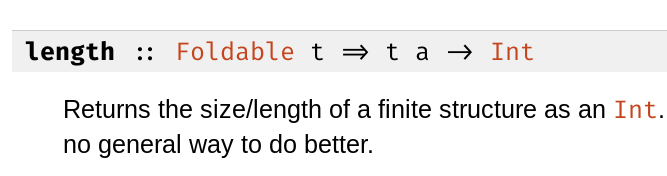
\includegraphics[width=0.5\textwidth]{figs/length.png}
      \caption{lol}
    \end{figure}
  }
  \frame{
    \frametitle{Exceptional negatives}
    Think of how many APIs return an ``\blueit{\texttt{Int}}''.
    \begin{enumerate}
      \item <2> How many of these APIs only use the negative numbers to signal errors?
    \end{enumerate}
  }
  \frame{
    \frametitle{What do we want?}
    If we think a bit about arithmetic we may conclude the following:
    \begin{enumerate}
      \item<2 -> Ideally, our operators would be \blueite{total}
      \item<3 -> When possible, we want our operators to be \blueite{closed}
    \end{enumerate}
  }
  \begin{frame}[fragile]
    \frametitle{Why?}
    These properties, when combined, allow us to be confident that when we
    operate on two \verb-Nat-s, we get another \verb-Nat-.
    \begin{enumerate}
      \item<2 -> This isn't true for arithmetic over all number systems (nor should it be!)
      \item<3 -> Many languages fail even where it should be!
    \end{enumerate}
  \end{frame}
  \frame{
    \frametitle{Totality}
    Our functions being \blueite{total} gives us confidence that for any input, we
    get a result.
  }
  \frame{
    \frametitle{Closure}
    Our functions being \blueite{closed} means that the result values lie within the
    same number system as their arguments.
  }
  \frame{
    \frametitle{What do we want? (part 2)}
    \myquote{The aim is a total closed system of arithmetic with results that
             can be safely interpreted in the context of the discrete
             structures in general programming}{Colin Runciman}{1989}
  }
  \frame{
    \frametitle{Back to arithmetic}
    Addition and Multiplication present no difficulties.
  }
  \frame{
    \frametitle{Back to arithmetic}
    What about Subtraction?
  }
  \begin{frame}[fragile]
    \frametitle{Don't wait, saturate}
  \end{frame}
  \begin{frame}[fragile]
    \frametitle{Don't wait, saturate}
    \begin{figure}
    {\color{dark-gray}
      \centering
\begin{BVerbatim}
(.-.) : Nat -> Nat -> Nat
n        .-.        Z = n
Z        .-.        _ = Z
(Succ n) .-. (Succ m) = n .-. m
\end{BVerbatim}
    }
    \end{figure}
  \end{frame}
  \frame{
    \frametitle{Relate back to data structures}
  }
  \begin{frame}[fragile]
    \frametitle{Relate back to data structures}
    \begin{figure}
    {\color{dark-gray}
      \centering
\begin{BVerbatim}
drop : Nat -> List a -> List a
drop Z        xs      = xs
drop _        []      = []
drop (Succ n) (x::xs) = drop n xs
\end{BVerbatim}
    }
    \end{figure}
  \end{frame}
  \begin{frame}[fragile]
    \frametitle{Relate back to data structures}
    We \emph{want} a correspondence between operations on data structures and
    on numbers:
    \begin{figure}
    {\color{dark-gray}
      \centering
\begin{BVerbatim}
length (drop n xs) === length xs .-. n
\end{BVerbatim}
    }
    \end{figure}
  \end{frame}
  \frame{
    \frametitle{Relate back to data structures}
    These sorts of correspondences are what we use (often in our head) when
    programming or refactoring.
  }
  \frame{
    \frametitle{A divisive issue}
    Unlike Subtraction, division is \emph{already} closed over Natural Numbers
  }
  \frame{
    \frametitle{A divisive issue}
    Unlike Subtraction, division is \emph{already} closed over Natural Numbers
    (for the cases for which it is defined!)
  }
  \frame{
    \frametitle{Back to square zero}
    Some mathematicians define the Natural Numbers as starting from One! Would
    that save us from this issue?
  }
  \frame{
    \frametitle{Back to square zero}
    Maybe, but then we'd lose the important correspondence with real data
    structures.
  }
  \frame{
    \frametitle{Quick digression}
  }
  \frame{
    \frametitle{Quick digression}
    Zero is not nothing!
  }
  \frame{
    \frametitle{Two solutions}
    Runciman proposes two solutions to the `division by zero' problem:
    \begin{enumerate}
      \item<2 -> based on viewing division on $\mathbb{N}$s as `slicing'
      \item<3 -> based on using lazy \texttt{Nat}s
    \end{enumerate}
  }
  \frame{
    \frametitle{Division as slicing}
    Think of dividing \texttt{x} by \texttt{y} as cutting \texttt{x} in
    \texttt{y} places.
  }
  \begin{frame}[fragile]
    \frametitle{Division as slicing}
    We can write a total division, \texttt{//}, in terms of a partial (fails when dividing by zero)
    division, \texttt{/}:
    \begin{figure}
    {\color{dark-gray}
      \centering
\begin{BVerbatim}
  
\end{BVerbatim}
    }
    \end{figure}
  \end{frame}
  \begin{frame}[fragile]
    \frametitle{Division as slicing}
    We can write a total division, \texttt{//}, in terms of a partial (fails when dividing by zero)
    division, \texttt{/}:
    \begin{figure}
    {\color{dark-gray}
      \centering
\begin{BVerbatim}
x // y = x / (Succ y)
\end{BVerbatim}
    }
    \end{figure}
  \end{frame}
  \frame{
    \frametitle{Umm...}
    We get one intuitive property
    \begin{itemize}
      \item<2 -> Slicing zero times gets you the original thing back
    \end{itemize}
  }
  \frame{
    \frametitle{... that's wrong}
    At the cost of it being \emph{incorrect} at every other \texttt{Nat}
  }
  \begin{frame}[fragile]
    \frametitle{Let's fix it}
    We get back correctness by subtracting $1$ from the divisor before passing it
    \texttt{//}
    \begin{figure}
    {\color{dark-gray}
      \centering
\begin{BVerbatim}
x ./. y = x // (y .-. 1)
\end{BVerbatim}
    }
    \end{figure}
  \end{frame}
  \frame{
    \frametitle{You coward!}
  }
  \frame{
    \frametitle{You coward!}
    In a sense we've only side-stepped the problem!
    \begin{itemize}
      \item<2 -> If you think this is the lazy solution...
    \end{itemize}
  }
  \frame{
    \frametitle{Even lazier}
    Runciman proposes another solution to this problem:
    \begin{itemize}
      \item<2 -> Lazy Natural Numbers
    \end{itemize}
  }
  \begin{frame}[fragile]
    \frametitle{Lazy \texttt{Nat}s}
    If we're in a lazy language we can have infinite structures!
    \begin{figure}
    {\color{dark-gray}
      \centering
\begin{BVerbatim}
 
\end{BVerbatim}
    }
    \end{figure}
  \end{frame}
  \begin{frame}[fragile]
    \frametitle{Go infinity...}
    If we're in a lazy language we can have infinite structures!
    \begin{figure}
    {\color{dark-gray}
      \centering
\begin{BVerbatim}
infinity = Succ infinity
\end{BVerbatim}
    }
    \end{figure}
  \end{frame}
  \begin{frame}[fragile]
    \frametitle{Back to division}
    \begin{figure}
    {\color{dark-gray}
      \centering
\begin{BVerbatim}
x ./. 0 = infinity
x ./. y = x / y
\end{BVerbatim}
    }
    \end{figure}
  \end{frame}
  \begin{frame}[fragile]
    \frametitle{No cheating}
    \begin{figure}
    {\color{dark-gray}
      \centering
\begin{BVerbatim}
                  
                
                                     
\end{BVerbatim}
    }
    \end{figure}
  \end{frame}
  \begin{frame}[fragile]
    \frametitle{No cheating}
    \begin{figure}
    {\color{dark-gray}
      \centering
\begin{BVerbatim}
x ./. y = if x < y
          then 0
          else Succ ((x .-. y) ./. y)
\end{BVerbatim}
    }
    \end{figure}
  \end{frame}
  \begin{frame}[fragile]
    \frametitle{More power to you}
    Exponentiation is not closed over the Integers, but over Naturals it is!
    \begin{figure}
    {\color{dark-gray}
      \centering
\begin{BVerbatim}
                  
                            
\end{BVerbatim}
    }
    \end{figure}
  \end{frame}
  \begin{frame}[fragile]
    \frametitle{More power to you}
    Exponentiation is not closed over the Integers, but over Naturals it is!
    \begin{figure}
    {\color{dark-gray}
      \centering
\begin{BVerbatim}
pow n        0 = 1
pow n (Succ p) = n * pow n p
\end{BVerbatim}
    }
    \end{figure}
  \end{frame}
  \frame{
    \frametitle{Laziness, revisited}
    Let's not start a war here
  }
  \frame{
    \frametitle{Laziness, revisited}
    Infinite values also allow you to avoid `cheating' in some standard algorithms
  }
  \frame{
    \frametitle{Laziness, revisited}
    How many times have you seen \texttt{inf = 999999} in a graph algorithm?
  }
  \begin{frame}[fragile]
    \frametitle{Save yourself some computation}
    Are there more than $10$ people in your company?
    \begin{figure}
    {\color{dark-gray}
      \centering
\begin{BVerbatim}
                       
\end{BVerbatim}
    }
    \end{figure}
  \end{frame}
  \begin{frame}[fragile]
    \frametitle{Save yourself some computation}
    Are there more than $10$ people in your company?
    \begin{figure}
    {\color{dark-gray}
      \centering
\begin{BVerbatim}
... expensive > 10 ...
\end{BVerbatim}
    }
    \end{figure}
  \end{frame}
  \frame{
    \frametitle{Laziness, revisited}
    Lazy numbers let us compare the sizes of things without necessarily
    fully computing the size!
  }

%%%%%%%%%%%%%%%%%%%%%%%%%%%%%%%%%%%%%%%% 
%%% API
%%%%%%%%%%%%%%%%%%%%%%%%%%%%%%%%%%%%%%%% 

  \frame{
    \frametitle{Sign post}
    \begin{enumerate}
      \item Overview of the $\mathbb{N}$s themselves
      \item Programming with \texttt{Nat}
      \item Arithmetic with \texttt{Nat} and properties we care about
      \item \blueit{How does \texttt{Nat} influence API design?}
      \item Implementation concerns
      \item Beyond \texttt{Nat}
      \item Conclude
    \end{enumerate}
  }
  \frame{
    \frametitle{APIs}
    We've alredy defined an API for arithmetic, with various tradeoffs.
    \begin{enumerate}
      \item<2 -> Now let's define some non-arithmetic functions and see how
                 the \texttt{Nat}s guide us
    \end{enumerate}
  }
  \frame{
    \frametitle{Size}
    Size of structures is very straightforward
  }
  \begin{frame}[fragile]
    \frametitle{Size}
    \begin{figure}
    {\color{dark-gray}
      \centering
\begin{BVerbatim}
size : List elem -> Nat
size      [] = Z
size (x::xs) = Succ (size xs)
\end{BVerbatim}
    }
    \end{figure}
  \end{frame}
  \frame{
    \frametitle{Position/Index}
    Finding the index of a thing is a little more interesting
  }

  \begin{frame}[fragile]
    \frametitle{Position/Index: Mark 1}
    \begin{figure}
    {\color{dark-gray}
      \centering
\begin{BVerbatim}
position : elem -> List elem -> ??????????
                        
       
                   
               
            
                          
                       
\end{BVerbatim}
    }
    \end{figure}
  \end{frame}
  \begin{frame}[fragile]
    \frametitle{Position/Index: Mark 1}
    \begin{figure}
    {\color{dark-gray}
      \centering
\begin{BVerbatim}
position : elem -> List elem -> ??????????
position a xs = pos xs 0
  where
    pos (x::xs) n =
               
            
                          
                       
\end{BVerbatim}
    }
    \end{figure}
  \end{frame}
  \begin{frame}[fragile]
    \frametitle{Position/Index: Mark 1}
    \begin{figure}
    {\color{dark-gray}
      \centering
\begin{BVerbatim}
position : elem -> List elem -> ??????????
position a xs = pos xs 0
  where
    pos (x::xs) n =
      if a == x
      then n
      else pos xs (Succ n)
                       
\end{BVerbatim}
    }
    \end{figure}
  \end{frame}
  \begin{frame}[fragile]
    \frametitle{Position/Index: Mark 1}
    \begin{figure}
    {\color{dark-gray}
      \centering
\begin{BVerbatim}
position : elem -> List elem -> ??????????
position a xs = pos xs 0
  where
    pos (x::xs) n =
      if a == x
      then n
      else pos xs (Succ n)
    pos      [] n = ????
\end{BVerbatim}
    }
    \end{figure}
  \end{frame}
  \begin{frame}[fragile]
    \frametitle{Position/Index: Mark 1}
    \begin{figure}
    {\color{dark-gray}
      \centering
\begin{BVerbatim}
position : elem -> List elem -> Option Nat
position a xs = pos xs 0
  where
    pos (x::xs) n =
      if a == x
      then Some n
      else pos xs (Succ n)
    pos      [] n = None
\end{BVerbatim}
    }
    \end{figure}
  \end{frame}

  \frame{
    \frametitle{Thoughts: Mark 1}
    This is satisfying because we're explicit about the possibility of failure
  }

  \begin{frame}[fragile]
    \frametitle{Position/Index: Mark 2}
    It should really be \texttt{positions}!
    \begin{figure}
    {\color{dark-gray}
      \centering
\begin{BVerbatim}
                                         
                         
       
                   
               
                               
                          
                      
\end{BVerbatim}
    }
    \end{figure}
  \end{frame}
  \begin{frame}[fragile]
    \frametitle{Position/Index: Mark 2}
    It should really be \texttt{positions}!
    \begin{figure}
    {\color{dark-gray}
      \centering
\begin{BVerbatim}
positions : elem -> List elem -> List Nat
positions a xs = pos xs 0
  where
    pos (x::xs) n =
      if a == x
      then n :: pos xs (Succ n)
      else pos xs (Succ n)
    pos      [] n = []
\end{BVerbatim}
    }
    \end{figure}
  \end{frame}

  \frame{
    \frametitle{Thoughts: Mark 2}
    In a lazy language \texttt{positions} is strictly more flexible
  }
  \frame{
    \frametitle{Thoughts: Mark 1 \& 2}
    Mind the gap
    \begin{itemize}
      \item<2 -> There were none!
    \end{itemize}
  }

  \begin{frame}[fragile]
    \frametitle{sublist}
    Take the sublist of a list:
    \begin{figure}
    {\color{dark-gray}
      \centering
\begin{BVerbatim}
sublist m n = take (n - m+1) . drop m
\end{BVerbatim}
    }
    \end{figure}
  \end{frame}

  \begin{frame}[fragile]
    \frametitle{sublist}
    The \texttt{sublist} function has invariants that the user has to keep
    in mind
    \begin{figure}
    {\color{dark-gray}
      \centering
\begin{BVerbatim}
sublist m n = take (n - m+1) . drop m
\end{BVerbatim}
    }
    \end{figure}
    \begin{itemize}
      \item<2 -> What if \texttt{n < (m-1)}?
      \item<3 -> \texttt{take} would be passed a negative argument!
    \end{itemize}
  \end{frame}
  \begin{frame}[fragile]
    \frametitle{sublist}
    Fix is straightforward
    \begin{figure}
    {\color{dark-gray}
      \centering
\begin{BVerbatim}
sublist : Nat -> Nat -> List elem -> List elem
sublist 0        n = take n
sublist (Succ m) n = take (n .-. m) . drop (Succ m)
\end{BVerbatim}
    }
    \end{figure}
  \end{frame}

%%%%%%%%%%%%%%%%%%%%%%%%%%%%%%%%%%%%%%%% 
%%% Implementation
%%%%%%%%%%%%%%%%%%%%%%%%%%%%%%%%%%%%%%%% 

  \frame{
    \frametitle{Sign post}
    \begin{enumerate}
      \item Overview of the $\mathbb{N}$s themselves
      \item Programming with \texttt{Nat}
      \item Arithmetic with \texttt{Nat} and properties we care about
      \item How does \texttt{Nat} influence API design?
      \item \blueit{Implementation concerns}
      \item Beyond \texttt{Nat}
      \item Conclude
    \end{enumerate}
  }
  \frame{
    \frametitle{Issues}
    Why don't we see \texttt{Nat}s everywhere?
    \begin{itemize}
      \item<2 -> Language designers don't include them in the stdlibs
      \item<3 -> Concerns about performance
    \end{itemize}
  }

  \frame{
    \frametitle{\texttt{Int}eresting observation}
    Even languages that \emph{try} to have some sort of non-negative
    number end up tripping over themselves!
    \begin{itemize}
      \item<2 -> e.g. C with \texttt{size\_t} and \texttt{ssize\_t}
    \end{itemize}
  }
  \frame{
    \frametitle{I'm not making this up}
    \begin{figure}
      \centering
      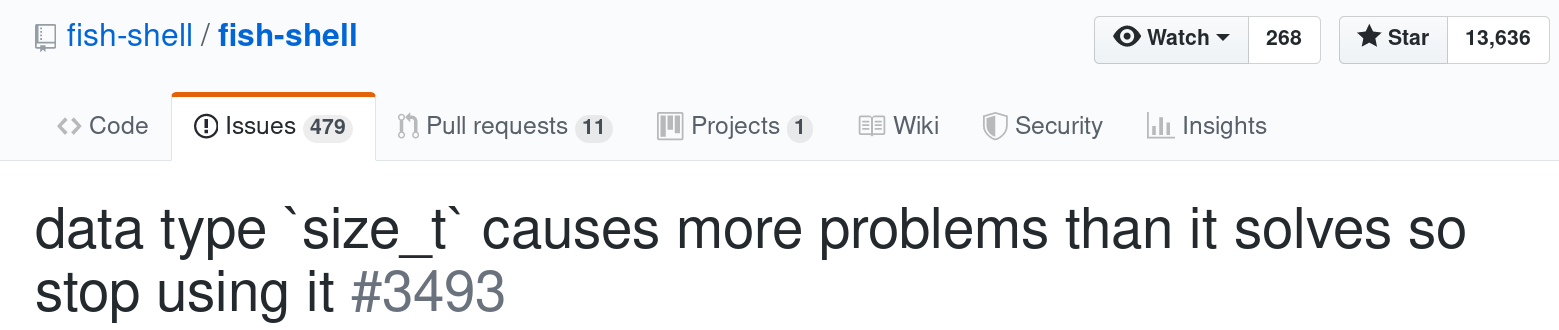
\includegraphics[width=\textwidth]{figs/fish-issue.png}
    \end{figure}
  }
  \frame{
    \frametitle{$\heartsuit$}
    \begin{figure}
      \centering
      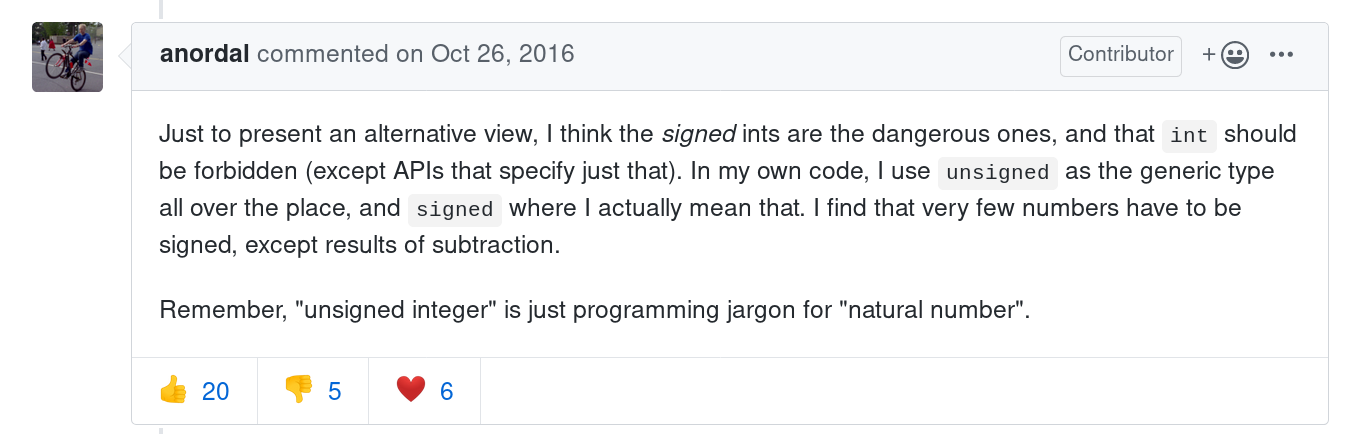
\includegraphics[width=\textwidth]{figs/love.png}
    \end{figure}
  }
  \frame{
    \frametitle{:'(}
    \begin{figure}
      \centering
      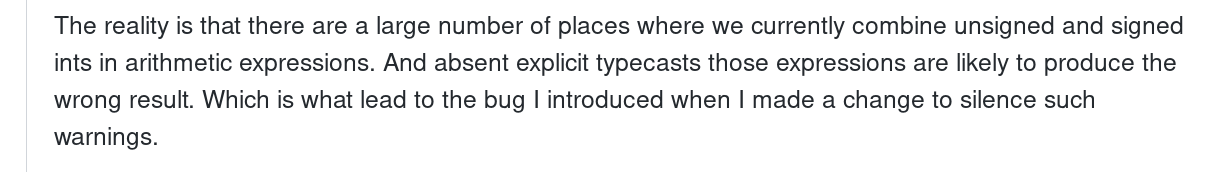
\includegraphics[width=\textwidth]{figs/reality.png}
    \end{figure}
  }
  \frame{
    \frametitle{Reality check}
    This person is not wrong!
    \begin{itemize}
      \item<2 -> understanding the behavior of casts (especially implicit ones) is hard!
    \end{itemize}
  }
  \frame{
    \frametitle{Is all hope lost?}
    The issue is twofold:
    \begin{itemize}
      \item<2 -> Unsigned values can be coerced away
      \item<3 -> Programmers aren't forced to recon with $0$!
    \end{itemize}
  }
  \frame{
    \frametitle{All hope is not lost}
    Some languages do it right!
    \begin{itemize}
      \item<2 -> Idris and Agda compile Peano \texttt{Nat}s to machine words
    \end{itemize}
  }
  \frame{
    \frametitle{What about the \emph{lazy} \texttt{Nat}s?}
    There are issues with implementing the lazy \texttt{Nat}s
    \begin{itemize}
      \item<2 -> Lazy languages can have poor memory usage if lazy structures
                 are implemented naively
    \end{itemize}
  }
  \frame{
    \frametitle{What about the \emph{lazy} \texttt{Nat}s?}
    What are the alternatives?
    \begin{enumerate}
      \item<2 -> a machine number
      \item<3 -> an unevaluated computation (i.e. a \emph{thunk})
      \item<4 -> a pair \texttt{(m,n)} of machine number and thunk
    \end{enumerate}
  }
  \frame{
    \frametitle{Why not machine?}
    \begin{enumerate}
      \item<2 -> Suitable for eager languages (IMO)
      \item<3 -> We lose \texttt{infinity} in lazy languages
    \end{enumerate}
  }
  \frame{
    \frametitle{Why not thunks?}
    \begin{enumerate}
      \item<2 -> Uses $O(n)$ space
      \item<3 -> where $n$ is the \blueite{value} of the \texttt{Nat}!
    \end{enumerate}
  }
  \frame{
    \frametitle{Perfect pair?}
    This leaves some combination of machine number and thunk
    \begin{enumerate}
      \item<2 -> Static analyses can help make it more efficient
      \item<3 -> `dirty' implementation techniques can be hidden from the user
    \end{enumerate}
  }

%%%%%%%%%%%%%%%%%%%%%%%%%%%%%%%%%%%%%%%% 
%%% Beyond Nat
%%%%%%%%%%%%%%%%%%%%%%%%%%%%%%%%%%%%%%%% 

  \frame{
    \frametitle{Sign post}
    \begin{enumerate}
      \item Overview of the $\mathbb{N}$s themselves
      \item Programming with \texttt{Nat}
      \item Arithmetic with \texttt{Nat} and properties we care about
      \item How does \texttt{Nat} influence API design?
      \item Implementation concerns
      \item \blueit{Beyond \texttt{Nat}}
      \item Conclude
    \end{enumerate}
  }

  \frame{
    \frametitle{What else}
    \begin{enumerate}
      \item<2 -> \texttt{Set}s!
    \end{enumerate}
  }

  \frame{
    \frametitle{Consider the following:}
    \begin{enumerate}
      \item<2 -> A function from an API you're using returns a \texttt{List}
      \item<3 -> Does order matter?
      \item<4 -> What does a duplicate element signal?
    \end{enumerate}
  }
  \frame{
    \frametitle{Mind the gap!}
    \begin{enumerate}
      \item<2 -> What if the same function returned a \texttt{Set}?
      \item<3 -> No order in the representation
      \item<4 -> No duplicate elements
    \end{enumerate}
  }
  \frame{
    \frametitle{Picking up the signals}
    \begin{enumerate}
      \item<2 -> Every data structure is signaling \blueite{something}
      \item<3 -> Asking the consumers of your API to \blueite{ignore} a signal
                 only serves to increas the cognitive burden of your API
      \item<4 -> Try choosing structures that are \blueite{necessary}
                 \emph{and} \blueite{sufficient}
      \item<5 -> This way, all signals are meant to be heeded
    \end{enumerate}
  }

%%%%%%%%%%%%%%%%%%%%%%%%%%%%%%%%%%%%%%%% 
%%% Conclusion
%%%%%%%%%%%%%%%%%%%%%%%%%%%%%%%%%%%%%%%% 

  \frame{
    \frametitle{Closing thoughts}
  }
  \frame{
    \frametitle{Closing thoughts}
    No one seems to disagree, and yet...
  }
  \frame{
    \frametitle{Ahead of his time}
  }
  \frame{
    \frametitle{Ahead of his time}
    \myquote{The benefits of lazy evaluation generally are now widely recognised
             (though still regarded as controversial by some)}{Colin Runciman}{The year of TS's birth}
  }


  \frame{
    \frametitle{Smash that subscribe button}
      Thanks for your time!

      You can read more of my rants \blueit{@josecalderon}
  }

  \frame {
    \centering {\fontsize{88}{68}\selectfont $\mathbb{N}$!}
  }

\end{document}
